\chapter{Entwicklung GraphQL-Service in .NET mit HotChocolate}
In diesem Kapitel wird die Entwicklung des Prototypen beschrieben.
Der Prototyp ist ein GraphQL-Service welcher mit .NET 6 und der Zuhilfenahme der Bibilothek HotChocolate entwickelt wurde.

\section{Anwendungsszenario}
% Der Anwendungsfall des Prototypen lässt sich wie folgt beschreiben:
% Da die Verwaltungen von Büchern und dazugehörige Autoren und Bewertungen ein aufwändiges Verfahren ist soll 
Die Auswahl eines neuen Buches ist oftmals ein sehr schwieriges Unterfangen.
Bei der Entscheidungsfindung helfen oft Bewertungen von Lesern, die das jeweilige Buch schon gelesen haben.
Demnach soll eine Bücher-Bewertungsplattform geschaffen werden.
Diese Plattform ermöglicht es Benutzern, Bücher zu bewerten und Informationen über Bücher, Autoren oder Bewertungen einzusehen.
% Benutzer, mit mehr Rechten als reinen Benutzerrechen, haben zudem die Möglichkeit die zusätzlich benötigten Entitäten 
Weiters sollen Benutzer in der Lage sein sich im System zu registrieren und anzumelden.
Angemeldete Benutzer haben, je nach ihren Benutzerrollen, Möglichkeiten im System verwaltete Entitäten zu Erstellen, zu Bearbeiten oder zu Löschen.

\section{Planung Schnittstelle}
Bevor ein Entwickler sich um die technische Umsetzung einer API kümmert, ist es ratsam, dass er sich einen Gesamtüberblick über das zu entwerfende System verschafft.
Dafür werden vor Beginn der technischen Umsetzung, unter Zuhilfenahme des Anwendungsszenarios, Use-Cases definiert.
% Diese Use-Cases definieren die Art und Weise wie ein Client auf den GraphQL-Service zugreif.
Diese Use-Cases beschreiben die benötigten Zugriffe eines Clients auf das System.
% Mit diesen Use-Cases definiert man wie ein Client auf den zukünftigen GraphQL-Service zugreift.
Zudem werden mit der Definition der Zugriffe auch die benötigen Entitäten definiert.
% Weiters erfolgt eine erste Definition der zu verwaltenden Objekte.
Aus dem Anwendungsszenario abgeleitete Use-Cases werden in der folgenden Abbildung grafisch dargestellt:

\begin{figure}[H]
    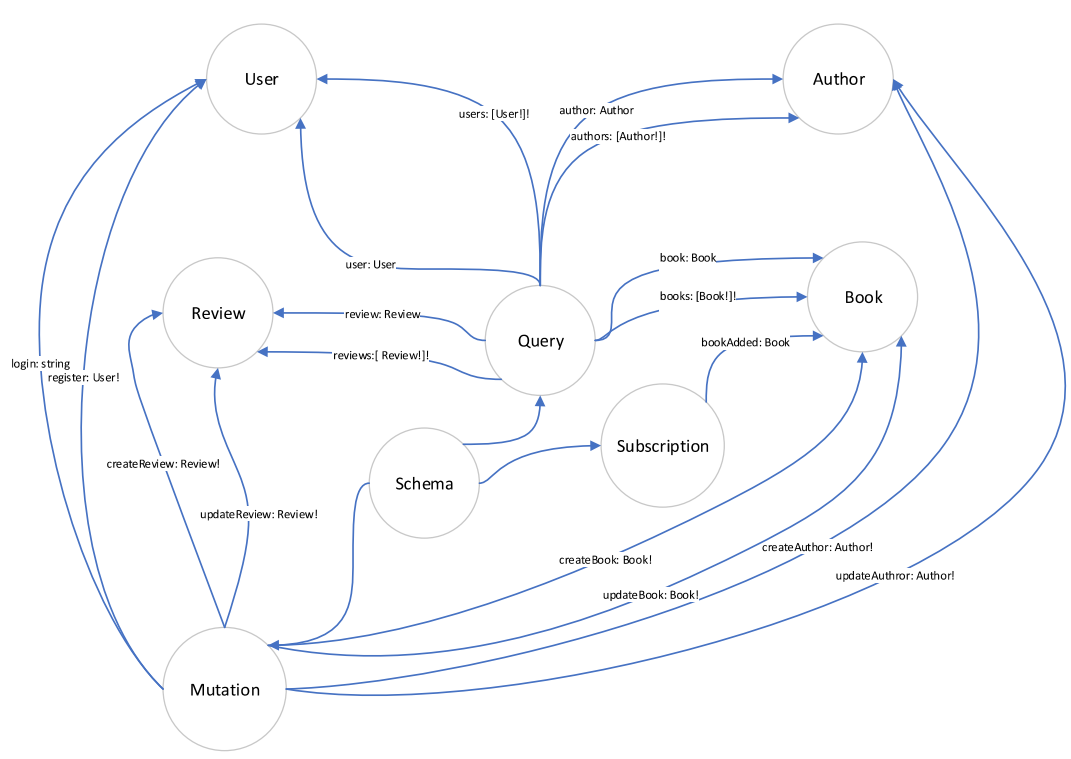
\includegraphics[width=\textwidth]{pics/graph_usecases.png}
    \caption{Use-Cases des Service.}
\end{figure}

Die obige Abbildung beschreibt die Zugriffsmöglichkeiten eines Clients auf den Prototypen.
Mit der Definition der Use-Cases geht auch die Definition der zu verwaltenden Entitäten einher.
Die zu vewaltenden Entitäten und ihre Relationen zueinander sind im folgenden ER-Diagram dargestellt:
% Weiters sind die Entitäten auf die Zugriffe möglich sind abgebildet.
% Dabei werden die Zugriffe jeweils
% Weiters zeigen die Use-Cases welche Entitäten im System zur Verfügung stehen werden.

% In der gezeigten Abbildung sieht man die vom Prototypen verwalteten Entitäten.
% Ebenso werden die lesenden und schreibenden Operationen auf diese dargestellt.

% Die zu verwaltenden  Relationen zwischen den Entitäten sind im folgenden ER-Diagram dargestellt:
\begin{figure}[H]
    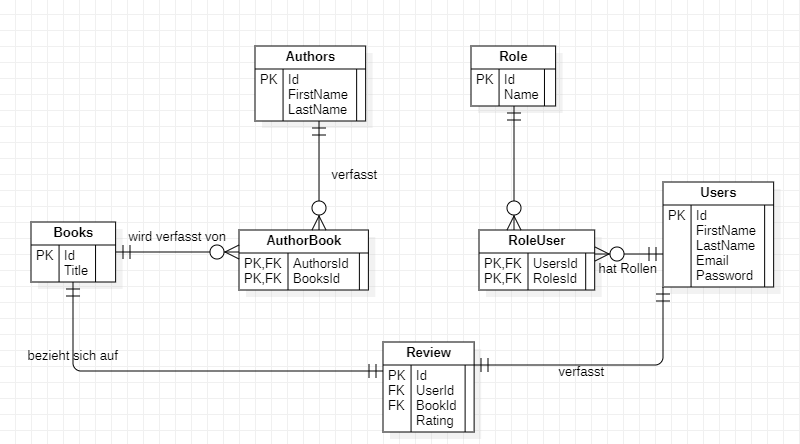
\includegraphics[width=\textwidth]{pics/ER-Diagram.png}
    \caption{Datenbankschema}
\end{figure}

\section{HotChocolate}
Für die Implementierung des GraphQL-Service wurde das Framework HotChocolate herangezogen.
Zusätzlich zum HotChocoalte Framework gibt es noch das .NET GraphQL Framework.
% Der Prototyp wurde aufgrund der steigenden Beliebtheit und Aktivät der Community des HotChocolate Frameworks mit eben jenem Framework umgesetzt.
Die Entscheidung, HotChocolate zu verwenden, fiel aufgrund der besseren Dokumentation des Frameworks und der höheren Aktivität der Community.

\myparagraph{HotChocolate Allgemein}
HotChoclate ist ein Open-Source Framework zur Implementierung eines GraphQL-Services.
Es ist konform, laut den GraphQL-Spezifikationen implementiert.
Damit ist HotChocolate kompatibel mit allen anderen GraphQL konform umgesetzten Clients.
Ein großer Teil der Komplexität, einen GraphQL-Service zu entwickeln, fällt dabei auf die Entwicklung des Schemas zurück.
HotChoclate kümmert sich um die Generierung des Schemas zur Laufzeit und entfernt somit einen großen Teil dieser Komplexität vom Entwickler.

\myparagraph{Schema Erstellung in HotChocolate}
Um das Schema in HotChocolate zu definieren gibt es 3 Varianten: \textit{Pure-Code-First}, \textit{Code-First} und \textit{Schema-First}.
Schema-First übernimmt dabei ein bereits bestehendes Schema und fügt es dem Service zu.
Code-First verwendet \textit{Attributes} um das Schema zu definieren.
Pure-Code-First verwendet eine Fluent-API.
Alle 3 Varianten liefern das selbe Schema, wobei man mit Pure-Code-First am meisten Kontrolle bei der Konfiguration hat.
Der Prototyp wurde mittels der Pure-Code-First Vorgehensweise umgesetzt.

\myparagraph{Dependency Injection}
Dependency-Injection in HotChocolate funktioniert sehr ähnlich wie die Dependency Injection von ASP.NET Applikationen.
Die Services werden wie üblich dem Dependency-Injection-Container hinzugefügt:

\begin{JsCode}
builder.Services.AddTransient(typeof(IRepository<>), typeof(Repository<>));
builder.Services.AddTransient(typeof(IBookRepository), typeof(BookRepository));
builder.Services.AddTransient(typeof(IAuthorRepository), typeof(AuthorRepository));
builder.Services.AddTransient(typeof(IReviewRepository), typeof(ReviewRepository));
builder.Services.AddTransient(typeof(IBaseService<>), typeof(BaseService<>));
builder.Services.AddTransient<IBookService, BookService>();
builder.Services.AddTransient<IAuthorService, AuthorService>();
builder.Services.AddTransient<IReviewService, ReviewService>();
builder.Services.AddTransient<IAuthService, AuthService>();
\end{JsCode}

HotChocolate unterstüzt dabei aber nicht die Constructor-Injection.
Stattdessen wird die Dependency-Injection in HotChoclate mittels Method-Dependency-Injection umgesetzt.
Würde man die Dependency-Injection mittels Constructor-Injection implementieren, so wäre jeder Service automatisch ein Singleton.
Für die Method-Injection liefert HotChocoalte das Attribute \textit{[Service]}.

Im folgenden Code-Beispiel ist die Verwendung ersichtlich:
\begin{JsCode}
public async Task<IQueryable<Book>> Books([Service]IBookService bookService) {
    //Execute Logic here
}
\end{JsCode}

\section{Architektur}
Der Prototyp wurde mit der für REST-APIs üblichen Drei-Schicht-Architektur umgesetzt.
Die Geschäftslogikschicht und Datenbankzugriffsschicht wurden dabei so entwickelt, dass die eigentlichen Implementierungen, je nach Bedarf, einfach ausgetauscht werden können.
% Auf die Geschäftslogik wird in den Unterkapiteln Query, Mutation und Subscription näher eingegangen. Die Datenbankzugriffsschicht wird im Kapitel Entity Framework näher erläutert.
\newline

\begin{figure}[H]
    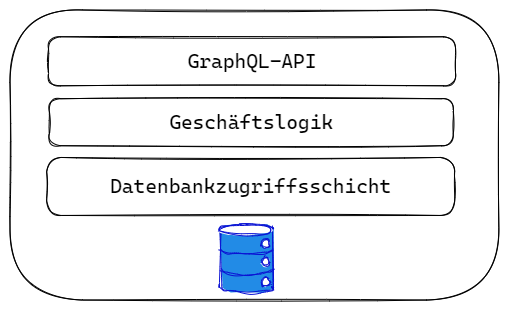
\includegraphics[width=\textwidth]{pics/architecture.png}
    \caption{Drei-Schicht-Architektur}
\end{figure}

Die hier abgebildete Architektur dient zur Veranschaulichung, die gezeigten Schichten werden in den folgenden Abschnitten näher erläutert.

\subsection{API:}
Die API bildet die einzige Schnittstelle des Systems zur Außenwelt.
Sie wird mittels dem GraphQL-Schema abgebildet.
Dieses Schema definiert, wie im GraphQL-Kapitel bereits erwähnt, die verfügbaren Typen sowie die lesenden und schreibenden Zugriffe des GraphQL-Service.

\subsection{Geschäftslogik}
Die Geschäftslogik bildet dabei die Logik der Server-Applikation ab.
Diese Logik wird dem GraphQL-Schema mittels Resolvern zur Verfügung gestellt.
Genaueres zu den Resolvern und zur Geschäftslogik folgt im Unterkapitel Resolver.
Die Geschäftslogik wurde mit dem DAO-Pattern umgesetzt und besteht aus \textit{Service} Klassen und zugehörigen Interfaces.

\subsection{Datenbankzugriff}
Die darunterliegende Datenbankzugriffsschicht ermöglicht, den darüberliegenden Schichten, CRUD-Operationen auf die angeforderten Daten auszuführen.
Für die Datenbankzugriffsschicht wurde dabei das Entity Framework verwendet.
Das Entity Framework ist ein \textit{Object Relational Mapper}, es ermöglicht Entwicklern den Fokus auf eine höhere Abstraktionsebene zu legen.
Diese Schicht wurde mit dem Repository-Pattern umgesetzt.
Wobei ein generisches Repository die Grundfunktionalität für die anderen entitätsspezifischen Repositories zur Verfügung stellt.

\section{Resolver}
Das Schema beschreibt, wie bereits im GraphQL-Kapitel erwähnt, nur die verfügbaren Typen, Querys, Mutations und Subscriptions.
Über die Generierung der Daten, als auch über die Manipulation dieser, hat das Schema kein Wissen.
Für den Datenzugriff bzw. Datenmanipulation sind in GraphQL \textit{Resolver} verantwortlich.
Jedes Feld in einer Query ist nichts anderes als eine Methode welches den Wert dieses Typs retourniert.
Jedes Feld eines Typs wird dabei einem \textit{Resolver} zugewiesen, diese Resolver sind Zugriffe auf die Geschäftslogik.
Wird ein Feld durch eine Query angefordert, liefert der jeweilige \textit{Resolver} die angeforderten Daten zurück.

\myparagraph{Umsetzung Resolver mittels Geschäftslogik}
Resolver werden im Prototypen durch die Geschäftslogik abgebildet, diese bieten CRUD-Operationen für die jeweilige Entität.
Jede Entität verfügt dabei über einen \textit{Service}.
Jeder Service wie zum Beispiel der \textit{AuthorService}, leitet dabei von einem generisch implementierten \textit{BaseService} ab.
Dieser \textit{BaseService} implementiert dabei das Interface \textit{BaseService}.
% Diese Services werden durch ein generisches \textit{Interface} \textit{IBaseService} und eine generische Basisimplementierung \textit{IBaseService} definiert.
\newline

\begin{JsCode}
public interface IBaseService<TEntity> where TEntity: BaseEntity {
    public Task<IQueryable<TEntity>> GetAsync(Expression<Func<TEntity, bool>> filter = null, params Expression<Func<TEntity, object>>[] includes);
    public Task<TEntity> GetFirstAsync(Expression<Func<TEntity, bool>> filter = null, params Expression<Func<TEntity, object>>[] includes);
    public Task<TEntity> AddAsync(TEntity entity);
    public Task<TEntity> UpdateAsync(TEntity entity);
    public Task<bool> ExistsAsync(int id);
    public Task RemoveAsync(TEntity entity);
}
\end{JsCode}

Im obigen CodeBeispiel ist das generische Interface \textit{IBaseService} abgebildet.
Es bietet Schnittstellen für die CRUD-Operationen jeder Entität.

\begin{JsCode}
public class BaseService<TEntity> : IBaseService<TEntity> where TEntity : BaseEntity {
    protected readonly IRepository<TEntity> repository;

    public BaseService(IRepository<TEntity> repository) {
        this.repository = repository;
    }
    public virtual async Task<IQueryable<TEntity>> GetAsync(Expression<Func<TEntity, bool>> filter = null, params Expression<Func<TEntity, object>>[] includes) {
        return await repository.GetAsync(filter, includes);
    }

    public virtual async Task<TEntity> GetFirstAsync(Expression<Func<TEntity, bool>> filter = null, params Expression<Func<TEntity, object>>[] includes) {
        return await repository.GetFirstAsync(filter, includes);
    }

    public virtual Task<TEntity> AddAsync(TEntity entity) {
        return repository.AddAsync(entity);
    }
    public virtual async Task<TEntity> UpdateAsync(TEntity entity) {
        return await repository.UpdateAsync(entity);
    }

    public virtual async Task<bool> ExistsAsync(int id) {
        return await repository.ExistsAsync(id);
    }

    public virtual async Task RemoveAsync(TEntity entity) {
        await repository.RemoveAsync(entity);
    }
}
\end{JsCode}

Im obigen Code-Beispiel ist die Basisimplementierung jedes Service zu sehen.
Besonders relevant für das Zusammenspiel mit HotChocolate ist dabei, dass die lesenden Operationen ein \textit{IQueryable} zurückliefern.
Warum \textit{IQueryable} so wichtig ist für HotChocolate wird im Abschnitt \textit{Field Middleware} näher erläutert.
\newline

Zusammenfassend lassen sich Resolver wie folgt zusammenfassen: Sie bieten den angefragten Feldern die benötigte Logik der Geschäftslogik um eben jene abgefragten Felder bereitzustellen.

%TODO Aufrufe relevant pagination -> projection -> filtering -> sorting
%todo die absätze aufeinander abstimmen erwähnen dass nur sortiert werden kann nachdem gefiltert wurde usw... bis nach oben hin
%sorting, filtering, projection ist ja nichts anders als middelware die nacheinander exekutiert wird, dabei Grafik von HotChocolate verwenden zur Veranschaulichung
\section{Field Middleware}
Field-Middleware erlaubt es, wiederverwendbare Logik vor oder nach der Exekution des Resolvers auszuführen.
% Diese Funktionalitäten sind Field-Middleware Komponenten von HotChocolate.
Funktionalitäten wie Authentifizierung / Autorisierung, Sortieren, Filtern, Pagination und Projection werden dabei von HotChocolate als Middlewarekomponenten zur Verfügung gestellt. 
Field-Middleware ist dabei \textit{composable}, somit kann man beliebig viele Middleware Komponenten aneinanderreihen.
Sie sind eine der fundamentalen Komponenten des Frameworks.

% Im folgenden Unterkapitel Query werden Funktionalitäten für das Authentifizieren und Autorisieren eines Benutzers als auch für das Sortieren, dem Filtern und der Projection verwendet.

\myparagraph{Reihenfolge Exekution Middleware}
Middlewarekomponenten werden in der Reihenfolge, in der sie definiert worden sind, ausgeführt.
Jede Middleware-Schicht kennt dabei nur die jeweils nächste Middleware.
Die letzte auszuführende Middleware ist dabei der eigentliche Resolver.
Die Reihenfolge der Anordnung der Middlewarekomponenten ist dabei sehr entscheidend, denn die Komponenten werden in genau dieser Reihenfolge exekutiert.
% Die Reihenfolge in der diese Middlewarekomponenten ausgeführt werden ist dabei sehr wichtig, denn sie entscheidet in welcher 
Die folgende Abbildung beschreibt die Aneinanderreihung der Middlewarekomponenten:

\begin{figure}[H]
    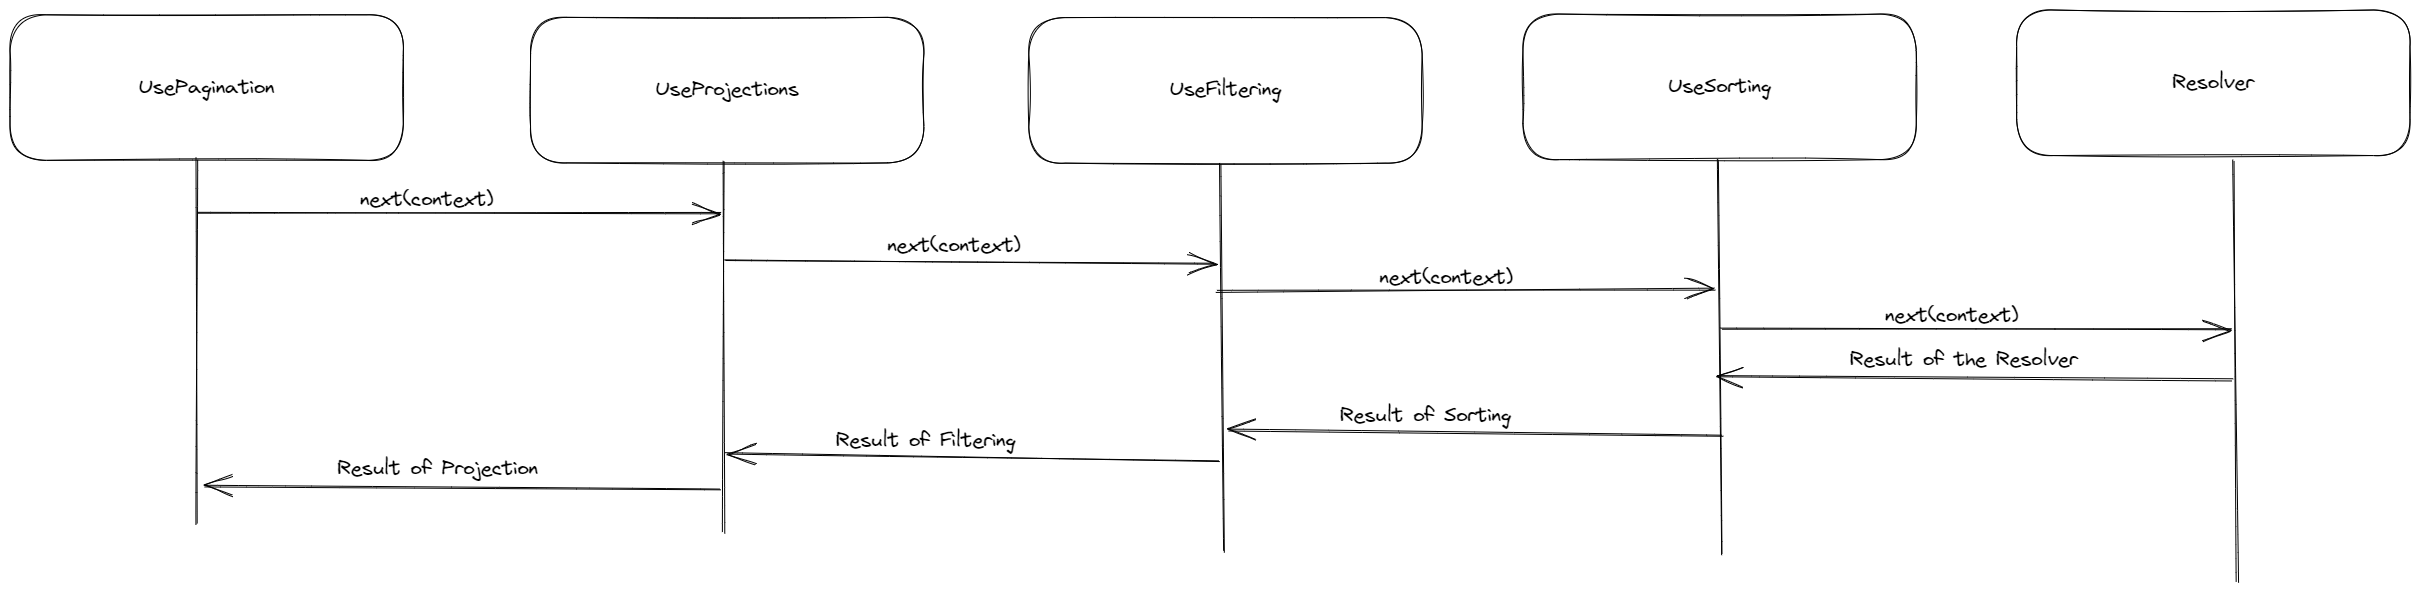
\includegraphics[width=\textwidth]{pics/middleware.png}
    \caption{Exekutierungsreihenfolge Middleware}
\end{figure}

In der obigen Abbildung ist zu sehen, dass die Middleware in der Reihenfolge ausgeführt wird, in der sie definiert wurde.
Das Resultat, welches von der letzten Middleware (dem Resolver) generiert wurde, wird in der umgekehrten Reihenfolge zurückgereicht.
Dabei wird das vom Resolver zurückgelieferte \textit{IQueryable} um die jeweiligen Operationen der restlichen Middlewarekomponenten erweitert.
\newline

Im Unterkapitel Query werden die verwendeten Middlewarekomponenten des Prototypen genauer erläutert.
% Da im Unterkapitel Query, welche die in der Implementierung, diese Middlewarekomponenten verwendet werden, erfolgt dort auch eine genauere Erläuterung der einzelnen Komponenten.
% In den folgenden Abschnitten wird auf zuvor erwähnten Middlewarekomponenten genauer eingegangen, diese sind für die folgenden Unterkapitel Query und Mutation von besonderer Relevanz: 

\myparagraph{Zusammenführung Middleware}
Nachdem jene Middleware, welche als erstes definiert wurde, das Ergebnis der restlichen Middlewarekomponenten erhalten hat wird das \textit{IQueryable} ausgeführt und das Ergebnis an den Client zurückgeliefert.

\section{Querys}
Im folgenden Abschnitt wird die Umsetzung, eines lesenden Zugriffs mittels einer Query, auf die Entität \textit{Author} erläutert.
Dabei wird das Zustandekommen der Schema-Definition der Query, als auch der Zugriff auf die Datenbank mittels der Geschäftslogik eingegangen.
Weiters wird erläutert wie HotChocolate das Over und Underfetching Problem löst, als auch Filtern, Sortieren und Pagination ermöglicht.
\newline
Die folgenden Unterkapitel widmen sich der Umsetzung der Query \textit{authors} welche alle im System gespeicherten Autoren liefert.
Dabei kann man diese Entitäten filtern, sortieren und paginieren. %TODO --> paginieren nicht so nice i guess

\myparagraph{Generierung Schema}
Um es einem Client zu ermöglichen auf die Autoren zuzugreifen, ist es erforderlich die Query im Schema zu definieren.
Hierbei wird für die Generierung des Schemas, das bereits erwähnte Pure-Code-First verwendet.
\newline

\begin{JsCode}
public class AuthorQuery: ObjectType<Query> {
    protected override void Configure(IObjectTypeDescriptor<Query> descriptor) {
        descriptor.Field("authors")
            .ResolveWith<AuthorResolver>(r => r.Authors())
            .Authorize()
            .UseProjection()
            .UseFiltering()
            .UseSorting()
            .Type<ListType<NonNullType<AuthorType>>>();
    }
}
\end{JsCode}

Im obigen Code-Beispiel ist zu sehen, dass die Wurzeloperation \textit{Query} um eine \textit{AuthorQuery} erweitert wird.
Überschreibt man nun die in der Klasse \textit{ObjectType} definierte Methode \textit{Configure} kann man die Felder der Query mit dem \textit{IObjectTypeDescriptor} erweitern.
Dabei wird das Feld \textit{authors} angelegt welches eine Liste von Autoren zurückgibt.

\begin{JsCode}
type Query{
    authors(where: AuthorFilterInput order: [AuthorSortInput!]): [Author!] @authorize(apply: BEFORE_RESOLVER)
}

type Author {
    firstName: String!
    lastName: String!
    books: [Book!]!
    id: Int!
}

input AuthorFilterInput {
    and: [AuthorFilterInput!]
    or: [AuthorFilterInput!]
    firstName: StringOperationFilterInput
    lastName: StringOperationFilterInput
    books: ListFilterInputTypeOfBookFilterInput
    id: ComparableInt32OperationFilterInput
}

input ListFilterInputTypeOfBookFilterInput {
  all: BookFilterInput
  none: BookFilterInput
  some: BookFilterInput
  any: Boolean
}

input AuthorSortInput {
    firstName: SortEnumType
    lastName: SortEnumType
    id: SortEnumType
}

input StringOperationFilterInput {
  and: [StringOperationFilterInput!]
  or: [StringOperationFilterInput!]
  eq: String
  neq: String
  contains: String
  ncontains: String
  in: [String]
  nin: [String]
  startsWith: String
  nstartsWith: String
  endsWith: String
  nendsWith: String
}

input ComparableInt32OperationFilterInput {
    eq: Int
    neq: Int
    in: [Int!]
    nin: [Int!]
    gt: Int
    ngt: Int
    gte: Int
    ngte: Int
    lt: Int
    nlt: Int
    lte: Int
    nlte: Int
}
\end{JsCode}

Der oben gegebene Code erzeugt dabei zur Laufzeit das hier gezeigte Schema.
% Das obige Code-Beispiel generiert dabei zur Laufzeit die im nächsten Code-Beispiel gezeigte Query.
Nur der \textit{AuthorType} als auch die Wurzel-Operation der Query mit dem Feld \textit{authors} wurden explizit generiert.
Die Methodenaufrufe \textit{Authorize()}, \textit{UseFiltering()} und \textit{UseSorting()} sind dabei für die Generierung von nicht explizit angegeben Typen verantwortlich.
Diese Methodenaufrufe aktivieren die jeweilige Field-Middleware, diese werden in den nachfolgenden Abschnitten genauer erläutert:

\myparagraph{Authorize}
Hierbei wird deklariert, dass nur angemeldete Benutzer Zugriff auf dieses Feld haben.
Diese Middleware ist, wie in der obigen Schemadefinition ersichtlich, vor dem Resolver auszuführen.
Sie stellt damit sicher, dass nur Anfragen mit einer gültigen Authentifizierung an die Geschäftslogik weitergereicht werden.
Im Schema wird das Feld \textit{authors} der Query mit der Direktive \textit{@authorize} versehen.
Näheres zur Authentifizierung und Autorisierung ist im gleichnamigen Abschnitt ersichtlich.

\myparagraph{Projection}
Mit \textit{Projections} liefert HotChocolate die Möglichkeit Over und Underfetching zu verhindern.
Over und Underfetching zu verhindern bedeutet, dass genau jene Daten, welche vom Client angefordert werden, in der Datenbank selektiert und anschließend an den Client zurückgeliefert werden.
Dabei bekommt HotChocolate vom \textit{Resolver} ein \textit{IQueryable}.
Dieses \textit{IQueryable} beinhaltet zunächst nur jene Filterungen und Selektionen welche von der Geschäftslogik festgelegt werden.
HotChocolate erweitert dieses \textit{IQueryable} nun durch jene Felder welche in der Query angefordert wurden.

\myparagraph{Filtering}
Aktiviert man die \textit{Filtering} Middleware für ein Query-Field, so kann man den implizit von HotChocolate bereitgestellten Filter-Input verwenden.
Diese Middleware erweitert das vom Resolver zurückgelieferte \textit{IQueryable} um die gegebene Filterung und liefert das Ergebnis der vorangestellten Middleware zurück.
Weiters ist es möglich benutzerdefinierte Typen für die Filterung zu definieren.

\myparagraph{Sorting}
Aktiviert man die \textit{Sorting} Middleware für ein Query-Field, so kann man den implizit von HotChocolate bereitgestellten Sortier-Input verwenden.
Diese Middleware fügt der vom Resolver zurückgelieferten \textit{IQueryable} die gegebene Sortierung hinzu.
Das Ergebnis wird wiederum an die vorangestellte Middleware zurückgeliefert.
Weiters ist es möglich benutzerdefinierte Typen für die Sortierung zu definieren.

\myparagraph{Zugriff auf Daten}
Der \textit{AuthorResolver} kümmert sich dabei um die Bereitstellung der geforderten Daten.
Er greift auf den \textit{AuthorService}, einer Kindklasse des \textit{BaseService}, zu und dieser mithilfe der Datenbankzugriffsschicht auf die Datenbank.
Wichtig dabei ist, dass der \textit{AuthorService}, HotChocolate ein \textit{IQueryable} zurückliefert.
Das zurückgelieferte \textit{IQueryable} wird vom Resolver an die restlichen Middlewarekomponenten zurückgereicht.
Diese erweitern dann das \textit{IQueryable} mit der von ihnen definierten Logik und werten es anschließend aus.

\myparagraph{Ausführung Query und Ergebnis}
\begin{figure}[H]
    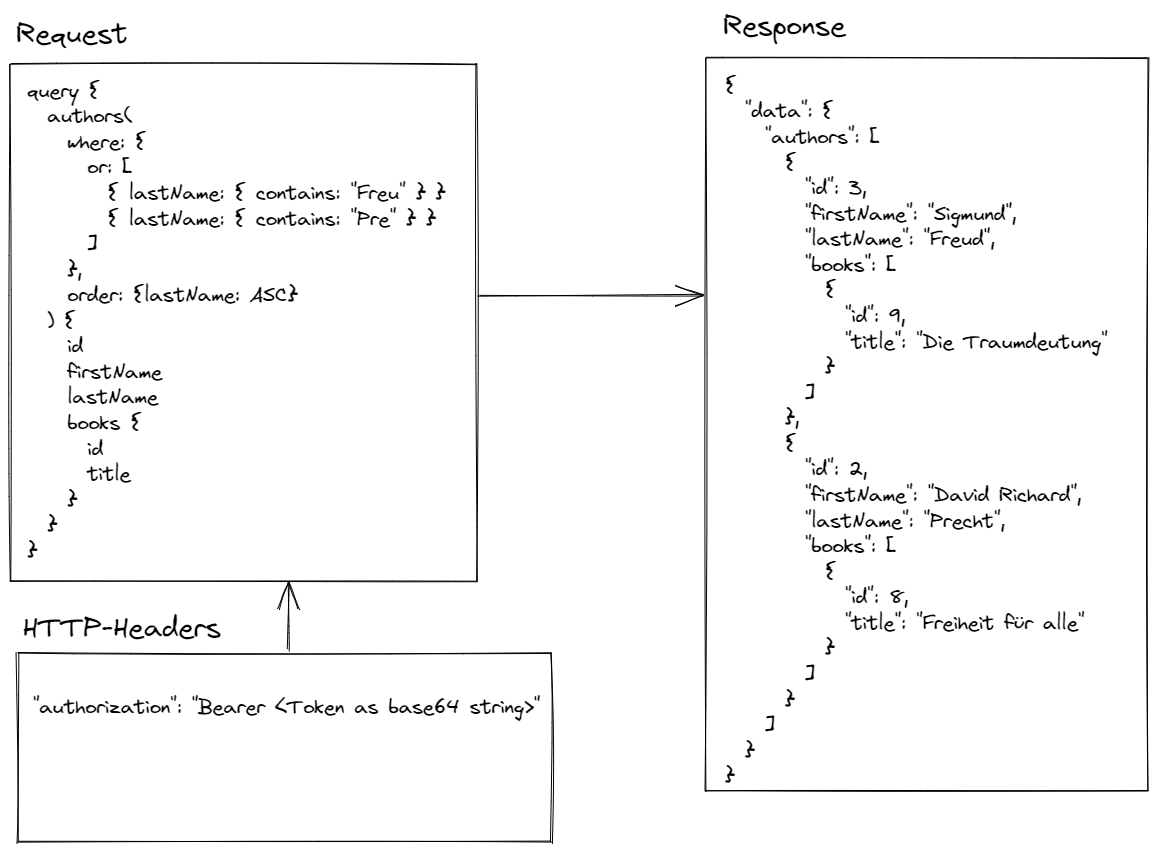
\includegraphics[width=\textwidth]{pics/authors_request.png}
    \caption{Exekutierungsreihenfolge Middleware}
\end{figure}

Die obige Abbildung zeigt eine Query, welche alle Autoren mittels dem Feld \textit{authors} abfrägt.
Dabei sollen nur jene Autoren zurückgegeben werden deren Nachname entweder "Freu" oder "Pre" enthält.
Weiters werden die Autoren nach ihrem Nachnamen sortiert.
Bei der Antwort des GraphQL-Service ist zu sehen, dass dieser die Daten genau in jenem Format zurückgibt, in dem sie angefragt worden sind.
Mittles HTTP-Parametern wurde der für die Authentifizierung notwendige \textit{JWT-Token} mitübermittelt.
\newline

Die oben abgebildete Anfrage hat am Server folgende Abfrage an die Datenbank ausgelöst:
\begin{JsCode}
SELECT [a].[Id], [a].[FirstName], [a].[LastName], [t].[Id], [t].[Title], [t].[AuthorsId], [t].[BooksId]
FROM [Authors] AS [a]
LEFT JOIN (
    SELECT [b].[Id], [b].[Title], [a0].[AuthorsId], [a0].[BooksId]
    FROM [AuthorBook] AS [a0]
    INNER JOIN [Books] AS [b] ON [a0].[BooksId] = [b].[Id]
) AS [t] ON [a].[Id] = [t].[AuthorsId]
WHERE ((@__p_0 LIKE N'') OR (CHARINDEX(@__p_0, [a].[LastName]) > 0)) OR ((@__p_1 LIKE N'') OR (CHARINDEX(@__p_1, [a].[LastName]) > 0))
ORDER BY [a].[LastName], [a].[Id], [t].[AuthorsId], [t].[BooksId]
\end{JsCode}

\section{Mutations}
Mutations werden wie bereits erwähnt für schreibende Zugriffe auf den GraphQL-Service verwendet.
In den folgenden Abschnitten wird die Umsetzung einer Mutation für das Bearbeiten eines bereits bestehenden Buches erläutert.
Dabei wird auf das Generieren des Schemas zur Laufzeit, als auch der Zugriff auf die Datenbank mittels der Geschäftslogik erläutert.

\myparagraph{Generierung Schema}
Damit ein Client die Möglichkeit hat auf eine Mutation zuzugreifen, muss der Wurzeloperation im Schema das gewünschte Feld hinzugefügt werden.
Dabei wird, wie bereits bei der Implementierung der Query, die Pure-Code-First Vorgehensweise angewendet.
\newline
Im folgenden Code wird die Wurzeloperation Mutation um ein Feld \textit{updateBook} erweitert.
Dabei werden nur Benutzern mit den Rollen Admin oder Bibliothekar die Ausführung gestattet.
Als Übergabeparameter bekommt die Funktion das \textit{DTO BookUpateInput}.
Der Resolver \textit{BookResolver} kümmert sich dabei um Ausführung der Operation.

\begin{JsCode}
public class BookMutation: ObjectTypeExtension<Mutation>{
    protected override void Configure(IObjectTypeDescriptor<Mutation> descriptor) {
        descriptor.Field("updateBook")
            .Authorize(new [] {"Admin", "Librarian"})
            .Argument("input", a => a.Type<NonNullType<BookUpdateInput>>())
            .ResolveWith<BookResolver>(r => r.UpdateBook(default, default))
            .Type<BookType>();
    }
}
\end{JsCode}

Der obige Code resultiert in folgendem Schema:
\begin{JsCode}
type mutation{
    updateBook(input: BookUpdateInput!): Book @authorize(roles: [ "Admin", "Librarian" ], apply: BEFORE_RESOLVER)
}

type Book {
  title: String!
  authors: [Author!]!
  reviews: [Review!]!
  id: Int!
}

type Author {
  firstName: String!
  lastName: String!
  books: [Book!]!
  id: Int!
}

type Review {
  userId: Int!
  user: User!
  bookId: Int!
  book: Book!
  rating: Int!
  id: Int!
}

type User {
  firstName: String!
  lastName: String!
  email: String!
  roles: [Role!]!
  reviews: [Review!]!
  id: Int!
}

type Role {
  name: String!
  users: [User!]!
  id: Int!
}

input BookUpdateInput {
  authors: [Int!]
  id: Int!
  title: String!
}
\end{JsCode}

In dem generierten Schema ist zu erkennen, dass der Objekt-Typ Buch alle Objekt-Typen die dieser explizit oder implizit referenziert, generiert wurden.
Desweiteren wurde die Wurzeloperation Mutation durch das Feld \textit{updateBook} erweitert.
Das Feld hat eine \textit{@authorize} Direktive, welche nur Benutzern mit den Rollen Admin oder Bibliothekar Zugriff gewährt.
Weiters wurde das Input-Objekt \textit{BookUpdateInput} generiert.
\newline

Das Input-Objekt \textit{BookUpateInput} wurde dabei zusätzlich wie folgt deklariert:
\begin{JsCode}
public class BookUpdateInput: InputObjectType<BookUpdate> {

    protected override void Configure(IInputObjectTypeDescriptor<BookUpdate> descriptor) {
        descriptor.Field(f => f.Authors).Type<ListType<NonNullType<IntType>>>();
    }
}

public class BookUpdate {
    public int Id { get; set; }
    public string Title { get; set; }
    public ICollection<int> Authors { get; set; }
}
\end{JsCode}

Bei der Definition des Input-Objekts \textit{BookUpdateInput} bietet die \textit{Configure} Methode der Basisklasse \textit{ObjectType} wiederum die Möglichkeit genauere Definitionen vorzunehmen.
Im obigen Code-Beispiel ist ersichtlich, dass das Feld \textit{Authors} eine Liste von \textit{Integer} enthält die nicht \textit{null} sein dürfen.
\newline

Anders als die im Datenbankschema beschriebene Entität Buch hält das Input-Objekt \textit{BookUdpateInput} keine Liste des Objekt-Typs Autor, sondern nur eine Liste von \textit{Integer} Werten, welche die IDs wiederspiegeln.
Mit dieser Vorgehensweise wird einer zyklischen Abhängigkeit vorgebeugt, denn sonst würden die Bücher Autoren referenzieren, welche wiederum Bücher referenzieren und das wiederholt sich endlos.
Um diese \textit{DTOs} wieder zu Domänenklassen umzuwandeln, müssen sie gemappt werden.
Dafür wird im Prototyp die Bibliothek \textit{AutoMapper} verwendet.

Im folgenden Code-Beispiel wird \textit{BookUpdateInput} wieder zu \textit{Book} umgewandelt:
\begin{JsCode}
public class BookProfile : Profile {
    public BookProfile() {
        CreateMap<BookUpdate, Book>()
            .ForMember(
            dest => dest.Authors,
            opt => opt.MapFrom(src => src.Authors.Select(id => new Author { Id = id })));
    }

}
\end{JsCode}

Zum Vergleich hier noch die Klasse \textit{Book} welche das Domänenobjekt Buch darstellt und von \textit{BaseEntity} ableitet und damit eine \textit{Id} erbt.

\begin{JsCode}
public class Book: BaseEntity {
    public string Title { get; set; }
    public List<Author> Authors { get; set; } = new List<Author>();
    public List<Review> Reviews { get; set; } = new List<Review>();
}
\end{JsCode}

\myparagraph{Ausführung und Ergebnis}

\begin{figure}[H]
    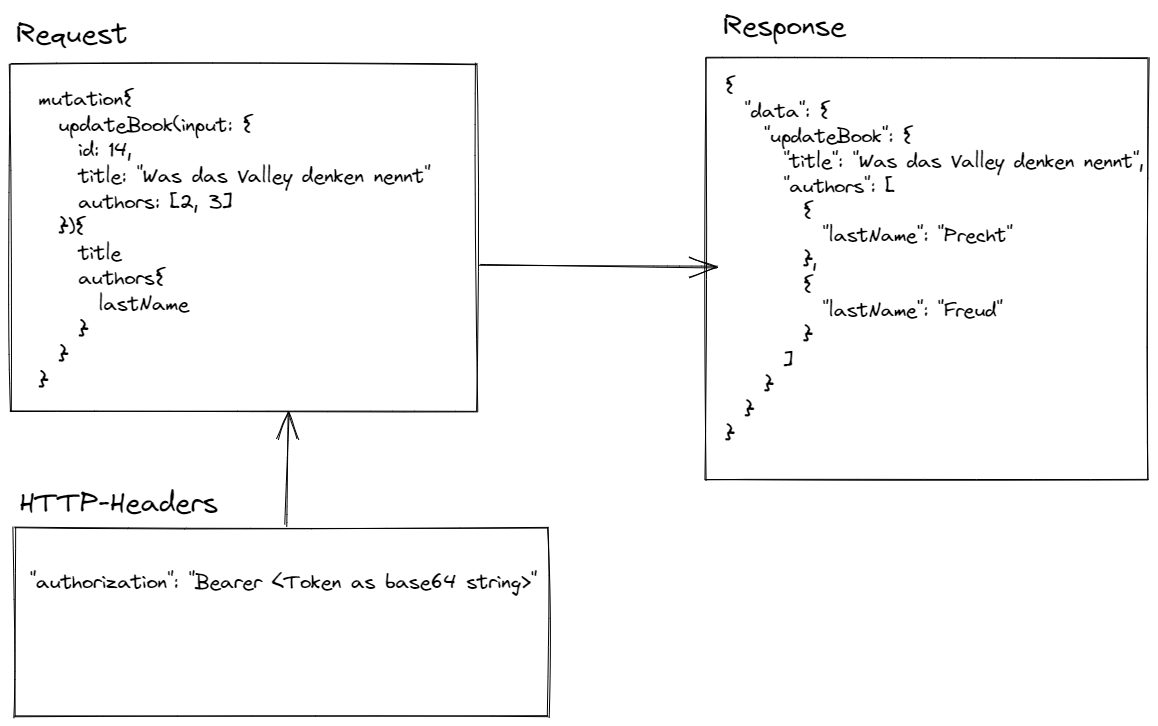
\includegraphics[width=\textwidth]{pics/execution_mutation.png}
    \caption{Schemadefinition}
\end{figure}

In dieser Abbildung ist die Ausführung des Feldes \textit{updateBook} der Mutation zu sehen.
Der Anfrage muss als HTTP-Header ein \textit{JWT-Token} übergeben werden um zu überprüfen ob der ausführende Benutzer genügend Rechte hat.
Die Antwort des GraphQL-Service entspricht dabei wiederum genau dem Schema welches in der Query der Anfrage angegeben wurde.


\section{Subscriptions}
Subscriptions werden wie bereits erwähnt verwendet, um bidirektionale Kommunikation zwischen dem Client und Server zu ermöglichen.
Dabei registriert sich der Client auf Events, welche vom Server ausgelöst werden, und bekommt dadurch in Echtzeit Updates.
HotChocolate realisiert Subscriptions mittels WebSockets.
HotChocolate bietet dabei 2 Subscription Provider: \textit{In-Memory} und \textit{Redis}.
Für den Prototypen wurde dabei die \textit{In-Memory} Version verwendet.

\myparagraph{Subscription über Event benachrichtigen}
Um eine Subscription über ein ausgeführtes Event zu benachrichtigen, stellt HotChocolate den \textit{ITopicEventSender} und den \textit{ITopicEventReceiver} zur Verfügung.
Diese Interfaces sind Abstraktionen der Funktionalitäten des Subscription Providers.
Diese Abstraktion ermöglicht es dem Entwickler, den Subscription Provider je nach Bedarf, zu einem späteren Zeitpunkt beliebig auszutauschen.
Um nun eine Subscription von einem Event zu benachrichtigen, ist folgender Code notwendig:
\begin{JsCode}
public async Task<Book> CreateBook([Service] IBookService bookService, BookCreate input,[Service] ITopicEventSender sender) {
    var book = await bookService.AddAsync(mapper.Map<Book>(input));
    await sender.SendAsync("bookAdded", book);
    return book;
}
\end{JsCode}

In Zeile 3 des obigen Code-Beispiels wird mittels dem \textit{ITopicEventSender} der \textit{ITopicEventReceiver} von dem neu erstelltem Buch notifiziert.
Auf die Verwendung des \textit{ITopicEventReceiver} wird in der folgenden Implementierung einer Subscription, welche auf die Erstellung eines Buches wartet, näher eingegangen:

\myparagraph{Schemagenerierung}
Für die Generierung des Schemas wird die Pure-Code-First Methode von GraphQL verwendet.
Die Wurzeloperationen Subscription wird dabei um ein Feld \textit{bookAdded} erweitert.
Die Umsetzung ist dabei in folgendem Code-Beispiel ersichtlich:

\begin{JsCode}
public class BookSubscription: ObjectTypeExtension<Subscription> {
    protected override void Configure(IObjectTypeDescriptor<Subscription> descriptor) {
        descriptor
        .Field("bookAdded")
        .Type<BookType>()
        .Resolve(context => context.GetEventMessage<Book>())
        .Subscribe(async context => {
            var receiver = context.Service<ITopicEventReceiver>();
            return await receiver.SubscribeAsync<string, Book>("bookAdded");
        });
    }
}    
\end{JsCode}
In Zeile 9 des obigen Code-Beispiels ist ersichtlich, dass der \textit{ITopicEventReceiver} auf eine Benachrichtigung durch den \textit{ITopicEventSender} wartet.

Der oben stehende Code generiert dabei folgendes Schema:
\begin{JsCode}
type subscription{
    bookAdded: Book
}

type Book {
  title: String!
  authors: [Author!]!
  reviews: [Review!]!
  id: Int!
}

type Author {
  firstName: String!
  lastName: String!
  books: [Book!]!
  id: Int!
}

type Review {
  userId: Int!
  user: User!
  bookId: Int!
  book: Book!
  rating: Int!
  id: Int!
}

type User {
  firstName: String!
  lastName: String!
  email: String!
  roles: [Role!]!
  reviews: [Review!]!
  id: Int!
}

type Role {
  name: String!
  users: [User!]!
  id: Int!
}
\end{JsCode} 

\myparagraph{Ausführung und Ergebnis}
Auf den Verbindungsaufbau von Subscriptions wurde bereits im Kaptiel GraphQL eingegangen.
Das folgende Bild zeigt das Ergebnis einer Subscription welche von der Erstellung eines Buches notifiziert wurde.

\begin{figure}[H]
    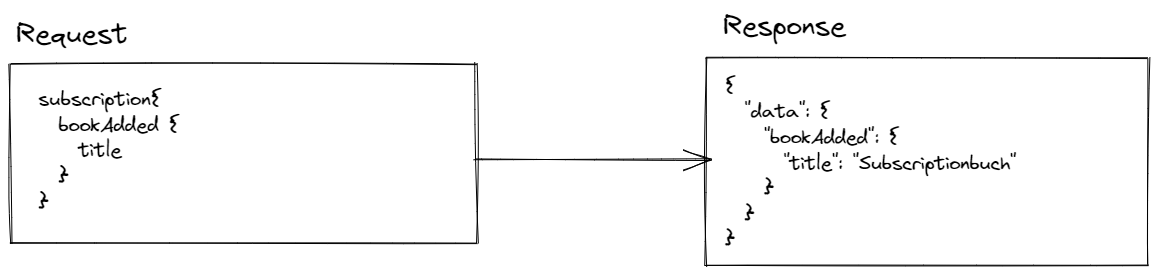
\includegraphics[width=\textwidth]{pics/bookSubscription.png}
    \caption{Subscription welche von der Erstellung eines Buches benachrichtigt wird.}
\end{figure}

\section{Authentifizierung und Autorisierung}
Als Authentifizierung wird jener Vorgang bezeichnet, mit dem die Identität eines Benutzers festgestellt wird.
Die Autorisierung wiederum ermittelt ob ein Benutzer die erforderlichen Rechte hat, um auf eine bestimmte Ressource zugreifen zu können.
Wie im Anwendungsszenario bereits beschrieben, gibt es im System 3 Rollen für Benutzer: User, Librarian und Admin.
Jede Rolle kann dabei nur für Sie freigegebene Ressourcen zugreifen.
\newline

Die Authentifizierung und Autorisierung für den Prototypen wird mit \textit{JWT-Tokens} und der Zuhilfenahme der \textit{ASP.NET Core-Authentifizierung} umgesetzt.
Die folgenden Abbildungen beschreiben die Rollen und die Ressourcen auf die sie Zugriff haben.
Grüne Felder bedeuten dabei, dass auch Benutzer ohne valides \textit{JWT-Token} Zugriff auf diese Ressource haben.
Das gelbe Feld "Einloggen" kann nur nach einer bereits erfolgten Registrierung aufgerufen werden.
Rote Felder wiederum verlangen ein valides \textit{JWT-Token} und sind an die Rolle des aufrufenden Benutzers gebunden.

\begin{figure}[H]
    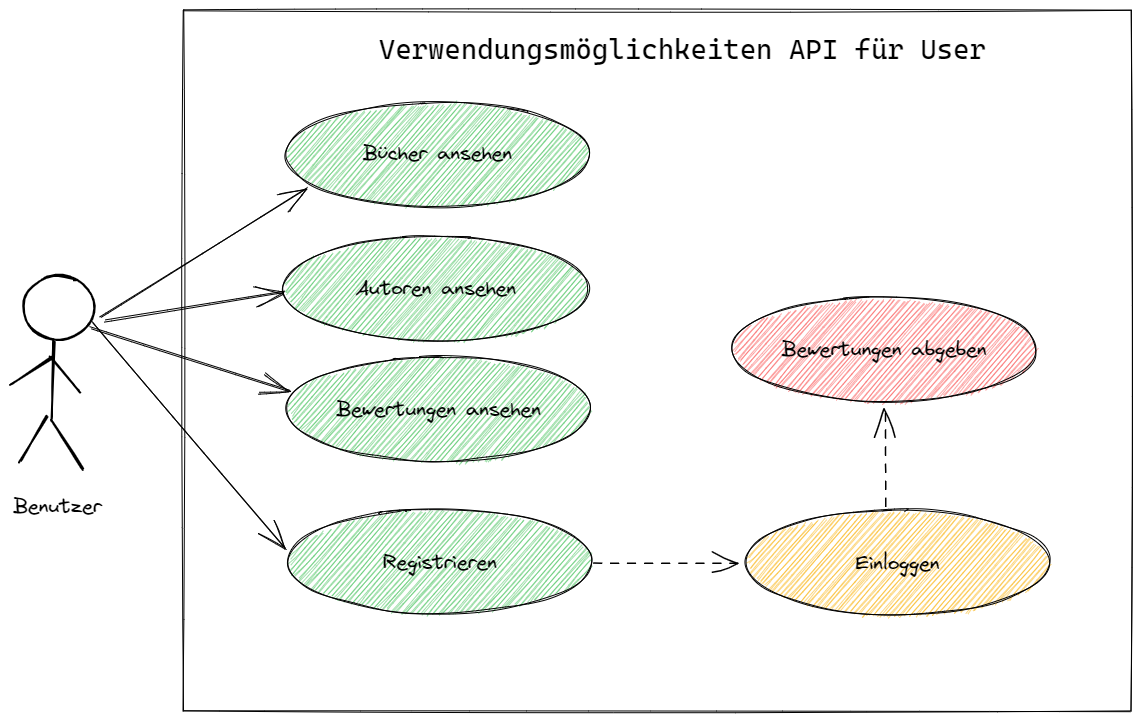
\includegraphics[width=\textwidth]{pics/UseCaseUser.png}
    \caption{Rechte User.}
\end{figure}

\begin{figure}[H]
    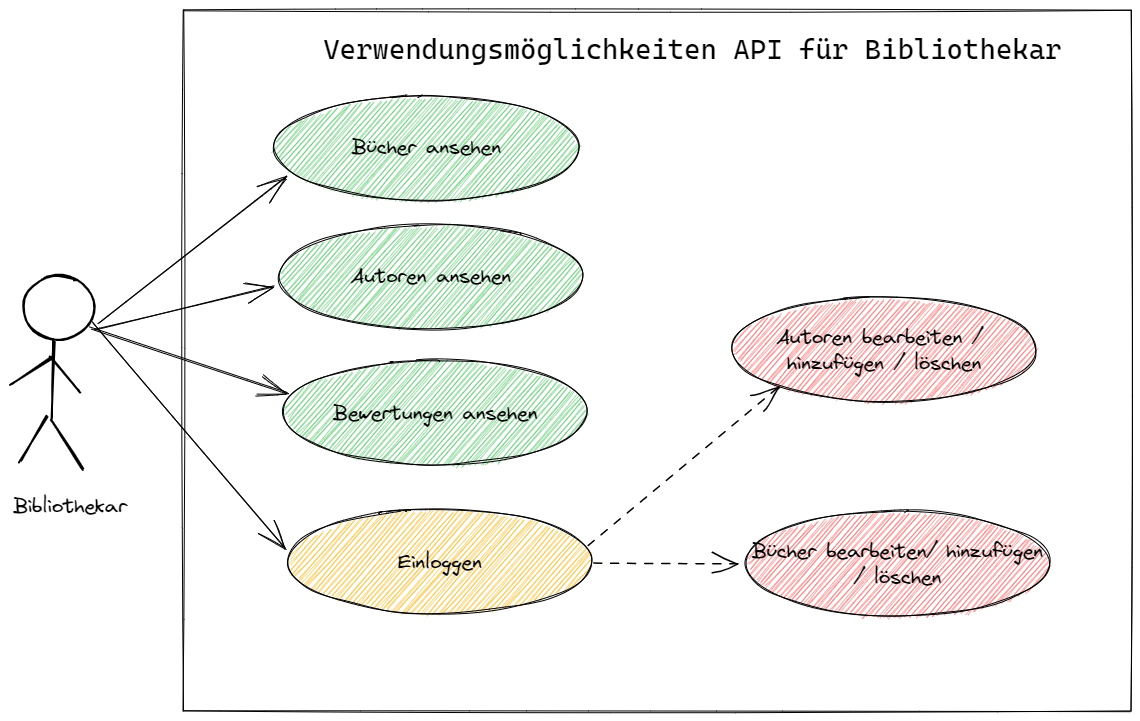
\includegraphics[width=\textwidth]{pics/UseCaseLibrarian.png}
    \caption{Rechte Bibliothekar.}
\end{figure}

\begin{figure}[H]
    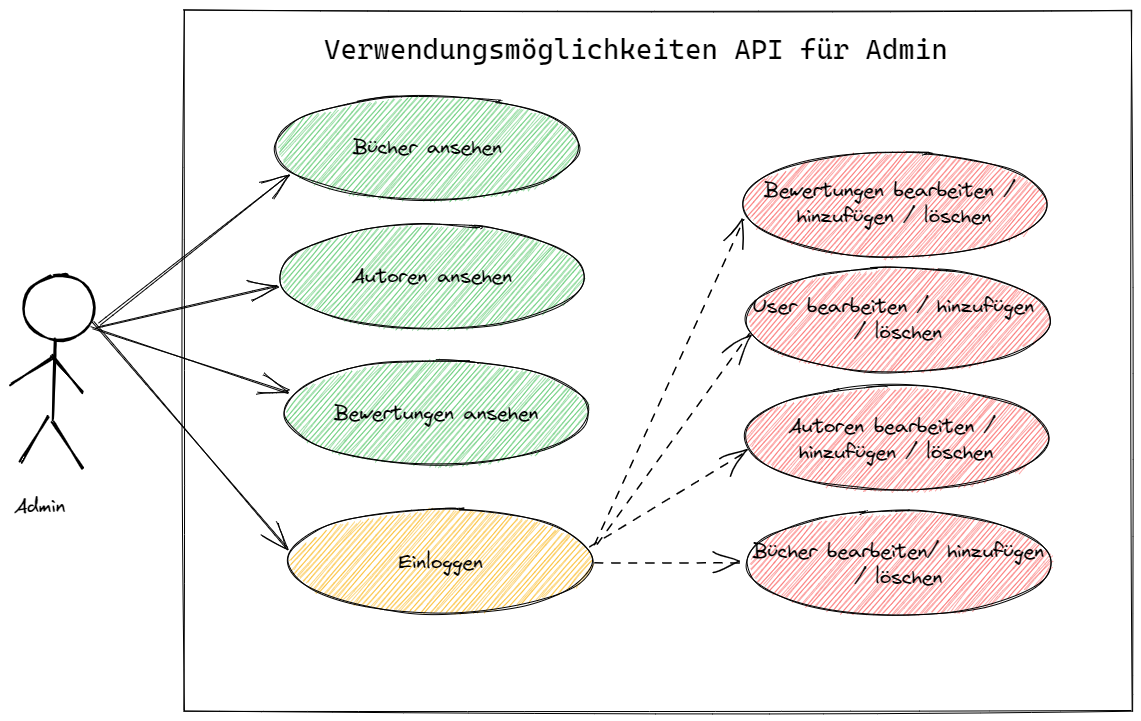
\includegraphics[width=\textwidth]{pics/UseCaseAdmin.png}
    \caption{Rechte Admin.}
\end{figure}

\myparagraph{Generierung JWT-Token}
Um die Authentifizierung mittels JWT-Token zu ermöglichen muss diese Authentifizierungsform erst registriert werden.
Diese Registrierung erfolgt, wie in .NET üblich, im \textit{WebApplicationBuilder}.

\begin{JsCode}
builder.Services.AddAuthentication(JwtBearerDefaults.AuthenticationScheme)
    .AddJwtBearer(options => {
        var tokenSettings = configuration
        .GetSection("JWT").Get<TokenSettings>();
        options.TokenValidationParameters = new TokenValidationParameters {
            ValidIssuer = tokenSettings.Issuer,
            ValidateIssuer = true,
            ValidAudience = tokenSettings.Audience,
            ValidateAudience = true,
            IssuerSigningKey = new SymmetricSecurityKey(Encoding.UTF8.GetBytes(tokenSettings.Key)),
            ValidateIssuerSigningKey = true
        };
    });
\end{JsCode}

Im obigen Code ist zu sehen, dass dem Server auf dem der GraphQL-Service läuft, eine JWT-Token Authentifizierung hinzugefügt wird.
Hierzu wurde eine Klasse \textit{TokenSettings} erstellt welche den \textit{Issuer}, die \textit{Audience} und den \textit{Key} welche die benötigten Daten aus der \textit{appsettings.json} liest und bereitstellt.
\newline

% Nachdem die zu verwendende Authentifizierungsmethode am Server registriert ist, ist es notwendig die Logik für die Erstellung eines Tokens zu implementieren.
Nach der Registrierung, der zu verwendenden Authentifizierungsmethode, erfolgt die eigentliche Generierung des Tokens.
Diese wurde im \textit{AuthService} in der Methode \textit{Login} umgesetzt.
Diese Methode erhält dabei einen Benutzernamen und ein Passwort als Übergabeparameter.
Hervorzuheben ist dabei, dass der Login als Mutation umgesetzt wurde.
Zum jetzigen Zeitpunkt finden keine schreibenden Operationen in dieser Methode statt.
Login-Operationen beinhalten aber oftmals das Speichern des Letzten erfolgreichen Logins, deswegen wurde für die Implementierung eine Mutation gewählt.
\newline

Im folgenden Code-Beispiel wird ein JWT-Token, bei übereinstimmenden User-Credentials, generiert.

\begin{JsCode}
public async Task<string> Login(string email, string password) {

    var user = await userRepository.GetFirstAsync(user => user.Email.Equals(email), user => user.Roles);
    if (user is not null && BCrypt.Net.BCrypt.Verify(password, user.Password)) {
        var securtityKey = new SymmetricSecurityKey(Encoding.UTF8.GetBytes(tokenSettings.Key));

        var credentials = new SigningCredentials(securtityKey, SecurityAlgorithms.HmacSha256);

        var claims = new List<Claim>();

        claims.Add(new Claim("FirstName", user.FirstName));
        claims.Add(new Claim("LastName", user.LastName));
        claims.Add(new Claim("Email", user.Email));
        if (user.Roles?.Count > 0) {
            foreach (var role in user.Roles) {
                claims.Add(new Claim(ClaimTypes.Role, role.Name));
            }
        }

        var jwtSecurityToken = new JwtSecurityToken(
            issuer: tokenSettings.Issuer,
            audience: tokenSettings.Audience,
            expires: DateTime.Now.AddDays(1),
            signingCredentials: credentials,
            claims: claims
        );

        return new JwtSecurityTokenHandler().WriteToken(jwtSecurityToken);
    }

    return "";
}
\end{JsCode}

Der obige Code beinhaltet die Überprüfung der vom Client übergebenen Benutzerdaten.
Stimmen diese mit jenen in der Datenbank überein, so wird ein JWT-Token generiert.
Der Token beinhaltet dabei folgende Daten des Benutzers: Vorname, Nachname, Email und die zugewiesenen Rollen.

\myparagraph{Verwendung Authentifizierung und Autorisierung}
Um ein Feld einer Query, Mutation oder Subscription nun abzusichern muss man die Field-Middleware Authentifizierung bei dem jeweiligen Feld aktivieren.
% Mit Pure-Code-First funktioniert das wie im folgenden Code-Beispiel abgebildet:
Mit der Pure-Code-First Methode von HotChocolate wird die Konfiguration in der \textit{Configure} Methode des jeweiligen \textit{ObjectType} abgebildet.

\begin{JsCode}
public class AuthorQuery: ObjectType<Query> {
    protected override void Configure(IObjectTypeDescriptor<Query> descriptor) {
        descriptor.Field("authors")
            .ResolveWith<AuthorResolver>(r => r.Authors())
            .Authorize()
            .Type<ListType<NonNullType<AuthorType>>>();
    }
}
\end{JsCode}

In dem oben stehenden Code wird festgelegt, dass ein User ein valides \textit{JWT-Token} an de Service übergeben muss um Zugriff auf die Ressource zu haben.
Im Umkehrschluss bedeutet dies, dass jeder Benutzer des Systems, wenn er angemeldet ist, Zugriff auf diese Ressource hat.
\newline

\begin{JsCode}
public class AuthorQuery: ObjectType<Query> {
    protected override void Configure(IObjectTypeDescriptor<Query> descriptor) {
        descriptor.Field("authors")
            .ResolveWith<AuthorResolver>(r => r.Authors())
            .Authorize(new [] {"Admin", "Librarian"})
            .Type<ListType<NonNullType<AuthorType>>>();
    }
}
\end{JsCode}
Dieser Code erweitert die erste Version um Autorisierung.
Es haben somit nur mehr Benutzer mit den Rollen Admin und Bibliothekar Zugriff auf diese Ressource.
Ein "normaler" Benutzer würde abgewiesen werden.

\section{1 + n Problem}
Lösung mit Dataloader


